\documentclass{article}
\usepackage[utf8]{inputenc}
\usepackage{xcolor}
\usepackage{amsmath}
\usepackage{scrextend}
\usepackage{listings}
\usepackage{tcolorbox}
\usepackage{graphicx}
\usepackage{tikz}
\usepackage{float}
\usepackage{hyperref}
\usepackage[framemethod=tikz]{mdframed}

\setlength{\parindent}{0pt}
\setlength{\parskip}{12pt}
\setlength{\intextsep}{0pt plus 2pt}

% For setting margins
\usepackage[margin=2in]{geometry}


\definecolor{codeColor}{HTML}{282c34}
\definecolor{keyWord}{HTML}{0000ff}
\definecolor{variable}{HTML}{ffffff}
\definecolor{CommentColor}{HTML}{aaaaaa}
\definecolor{StrColor}{HTML}{00ff00}
\definecolor{ruleColor}{HTML}{282c34}

\graphicspath{{.}}

\lstset{basicstyle=\small\footnotesize\color{variable},
        commentstyle=\color{CommentColor},
        stringstyle=\color{StrColor},
        breaklines=true, 
        showlines=false}


\title{Assignment 2}
\date{}
\author{Jonas Valfridsson\\199608275377}

\begin{document}

\maketitle
\tableofcontents

All the code of all the exercises can be found here:

\href{https://github.com/DD2360-Assignments-Jonas-Valfridsson/Assignments}{https://github.com/DD2360-Assignments-Jonas-Valfridsson/Assignments}

\section*{Hello World!}%
\label{sec:hello_world_}


Running the 'Hello World' program does not necessarily produce an ordered output. This is because the threads are not ran in any particular order. I am
executing my program on Ubuntu 16.04.6 LTS (Xenial Xerus) on my 1080 GTX TI, i compile the programs with: 


\begin{mdframed}[backgroundcolor=codeColor,leftmargin=0.0cm,hidealllines=true,%
  innerleftmargin=0.1cm,innerrightmargin=0.1cm,innertopmargin=0.5cm,innerbottommargin=0.10cm,
  roundcorner=15pt]
\begin{lstlisting}[language=bash]
function ccuda {
  nvcc -Xptxas -O3,-v  -std=c++11 -arch=sm_61  $1 -o $2
}
\end{lstlisting}
\end{mdframed}


\subsubsection*{The Execution Model}%
\label{ssub:}

Each cuda kernel is executed on a grid. A grid consists of thread blocks, each thread block is executed by a SM. Each thread block contains a collection of
threads, each thread runs the kernel code.


\section*{SAXPY on GPU}%
\label{sec:saxpy_on_gpu}

I approached the problem of having input arrays that are not a multiple of my block size buy creating one extra block. In reality I don't always have to create
one extra block but for simplicity sake I did it in this assignment. Following is a benchmark of SAXPY CPU vs GPU:

\begin{figure}[H]
  \centering
  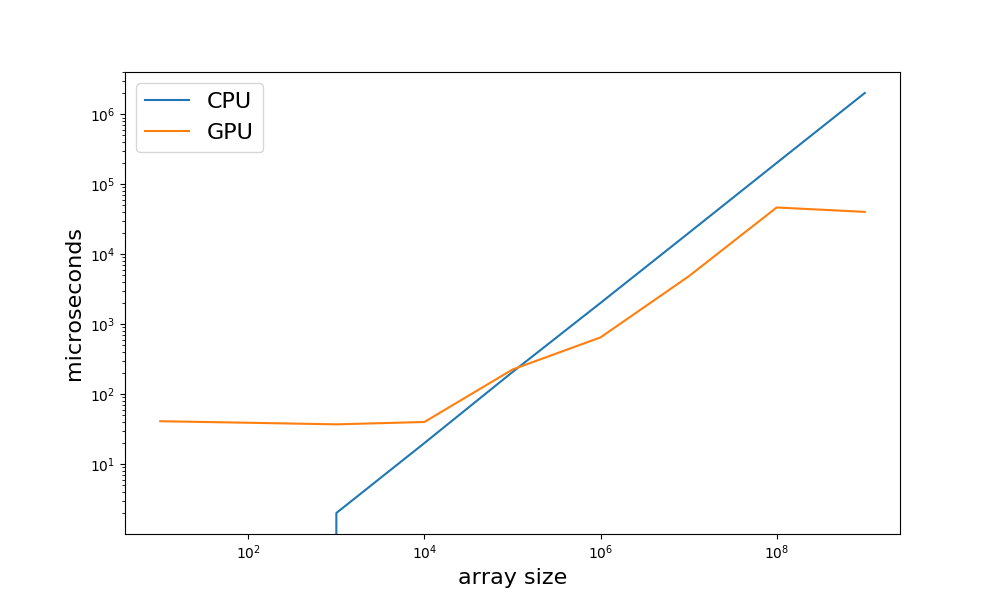
\includegraphics[width=0.95\linewidth]{ex_2/saxpy-cpu-vs-gpu.png}
  \label{fig:}
\end{figure}

Notice that the axes are in log-scale - At the final array size (1e9) the GPU is about 50x faster than CPU.

\section*{CUDA Simulation and GPU profiling}%
\label{sec:cuda_simulation_and_gpu_profiling}

\begin{figure}[H]
  \centering
  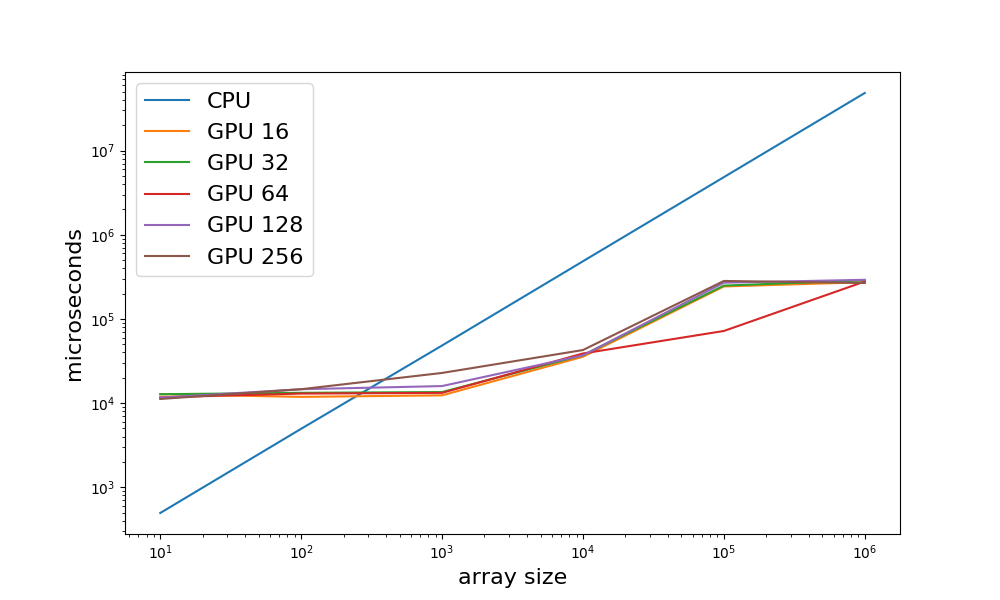
\includegraphics[width=0.95\linewidth]{ex_3/simulation-cpu-vs-gpu.png}
  \label{fig:}
\end{figure}


\textbf{3)}
I used the same GPU as before (1080GTX-ti) with same compilation command as above. I ran with 1000 time steps, the block-size did not really seem to matter.

\textbf{4)}
If particles would have needed to be copied back and forth at each time-step the program would have become about 3 * "number of time-steps" slower, meaning 300x
slower for me - this would make it slower than my CPU. So running running it on GPU would not be worth it if I had to copy for each time-step.


\section*{Calculate PI with CUDA}%
\label{sec:calculate_pi_with_cuda}

\begin{figure}[H]
  \centering
  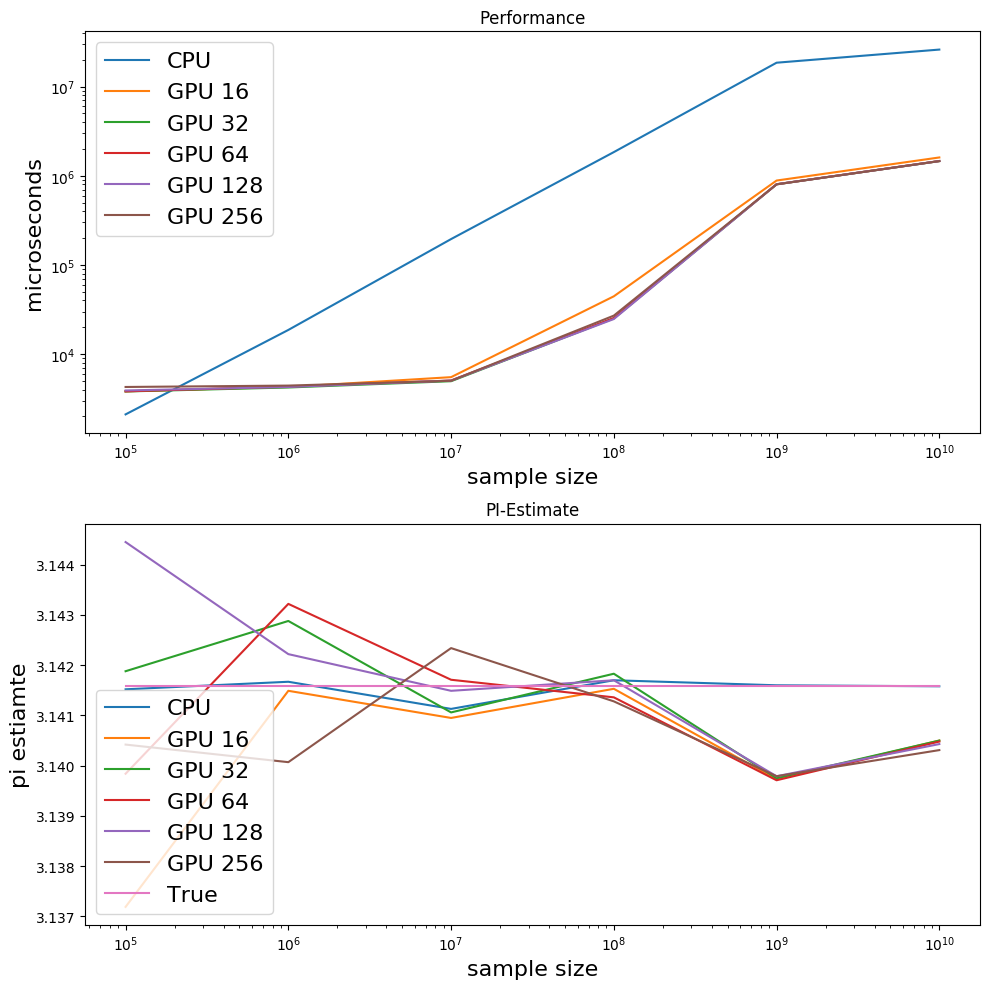
\includegraphics[width=0.95\linewidth]{ex_4/pi-float-cpu-vs-gpu.png}
  \caption{single precision}
  \label{fig:}
\end{figure}

\begin{figure}[H]
  \centering
  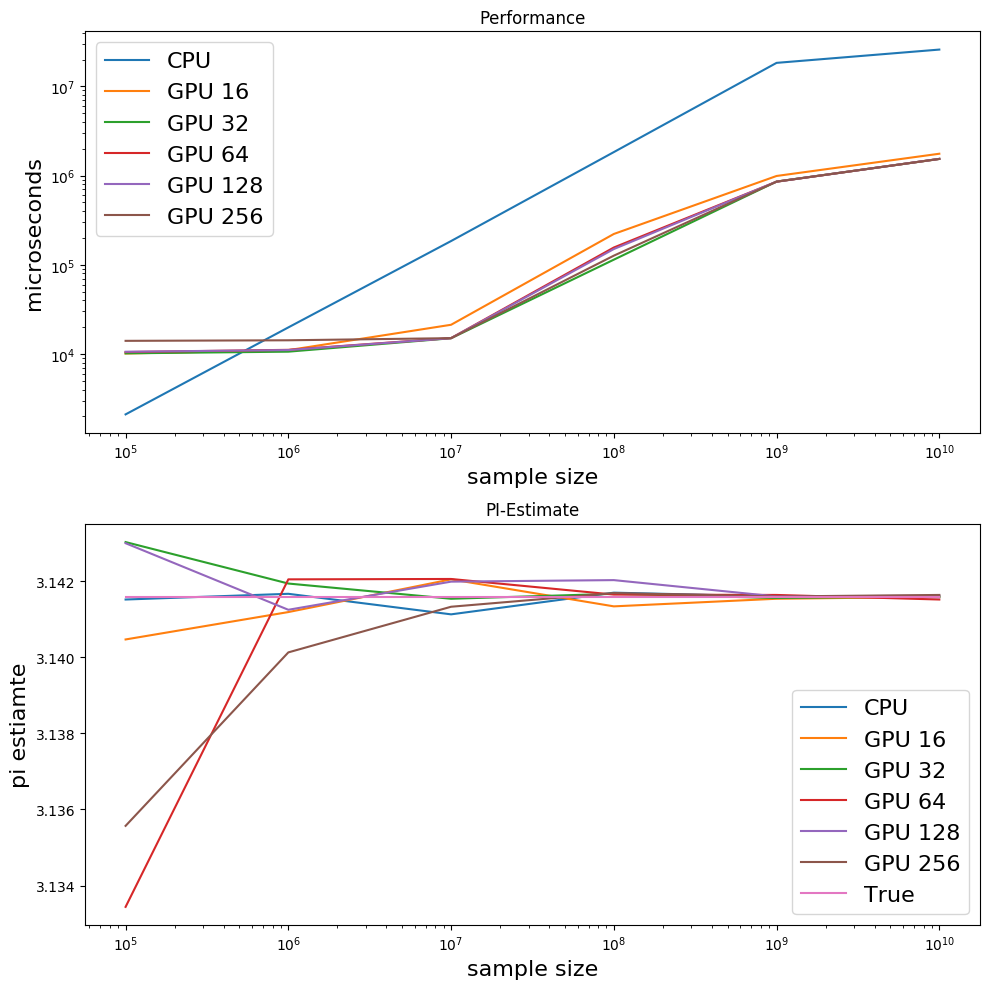
\includegraphics[width=0.95\linewidth]{ex_4/pi-double-cpu-vs-gpu.png}
  \caption{double precision}
  \label{fig:}
\end{figure}


The single precision was significantly faster, but due to my implementation it lost quite a bit of precision since I am averaging over threads at the end. The
double precision was fine with the averaging but was slower, as expected. The best case scenario would be to use mixed precision.

From the plots above it cant be seen that single-precision was faster, this is due to the fact that I always sampled 2000 samples per thread and when the sample
size was big ($> 1e9$) this ment I had many theads and the biggest bottleneck was then to setup the rng. In fact it took more than 90\% of the time

\begin{mdframed}[backgroundcolor=codeColor,leftmargin=0.0cm,hidealllines=true,%
  innerleftmargin=0.1cm,innerrightmargin=0.1cm,innertopmargin=0.5cm,innerbottommargin=0.10cm,
  roundcorner=15pt]
\begin{lstlisting}[language=bash]
==24413== ..: ./exercise_4 10000000000 2000 256
==24413== Profiling result:
Time(%)      Time     Calls       Avg   Name
 94.37%  1.44804s         1  1.44804s   setup_gpu_rng(..)
  5.52%  84.672ms         1  84.672ms   gpu_estimate_pi(..)
  0.11%  1.6563ms         1  1.6563ms   [CUDA memcpy DtoH]
 91.02%  1.53477s         1  1.53477s   cudaMemcpy
  8.74%  147.30ms         2  73.652ms   cudaMalloc
  0.19%  3.2549ms         2  1.6274ms   cudaLaunchKernel
  0.03%  489.38us         1  489.38us   cuDeviceTotalMem
  0.02%  333.56us        96  3.4740us   cuDeviceGetAttribute
  0.00%  36.231us         1  36.231us   cuDeviceGetName
  0.00%  15.117us         1  15.117us   cuDeviceGetPCIBusId
  0.00%  6.9090us         2  3.4540us   cuDeviceGet
  0.00%  2.0810us         3     693ns   cuDeviceGetCount
                    0.00%     374ns      374ns     374ns  cuDeviceGetUuid
\end{lstlisting}
\end{mdframed}

This could be mitigated by increasing the number of samples per thread, e.g 10000 samples with block size of 32 instead of 2000 samples with 256 seems to be a
sweet spot for 1e10 total samples. 

\begin{mdframed}[backgroundcolor=codeColor,leftmargin=0.0cm,hidealllines=true,%
  innerleftmargin=0.1cm,innerrightmargin=0.1cm,innertopmargin=0.5cm,innerbottommargin=0.10cm,
  roundcorner=15pt]
\begin{lstlisting}[language=bash]
==24907== ..: ./exercise_4 10000000000 10000 32
==24907== Profiling result:
 Time(%)      Time     Calls       Avg  Name
  91.91%  105.29ms         1  105.29ms  gpu_estimate_pi(..)
   8.01%  9.1746ms         1  9.1746ms  setup_gpu_rng(..)
   0.08%  87.713us         1  87.713us  [CUDA memcpy DtoH]
  55.58%  148.30ms         2  74.150ms  cudaMalloc
  42.92%  114.52ms         1  114.52ms  cudaMemcpy
   1.22%  3.2569ms         2  1.6284ms  cudaLaunchKernel
   0.15%  393.23us         1  393.23us  cuDeviceTotalMem
   0.12%  311.26us        96  3.2420us  cuDeviceGetAttribute
   0.01%  31.332us         1  31.332us  cuDeviceGetName
   0.01%  14.707us         1  14.707us  cuDeviceGetPCIBusId
   0.00%  1.6790us         3     559ns  cuDeviceGetCount
   0.00%  1.1440us         2     572ns  cuDeviceGet
   0.00%     306ns         1     306ns  cuDeviceGetUuid
\end{lstlisting}
\end{mdframed}

This is about 10x faster than the other GPU code which makes it more than 100x faster than the CPU code. Running it with float instead of double makes it about
10x faster again

\begin{mdframed}[backgroundcolor=codeColor,leftmargin=0.0cm,hidealllines=true,%
  innerleftmargin=0.1cm,innerrightmargin=0.1cm,innertopmargin=0.5cm,innerbottommargin=0.10cm,
  roundcorner=15pt]
\begin{lstlisting}[language=bash]
==25030== ..: ./exercise_4 10000000000 10000 32
==25030== Profiling result:
Time(%)      Time     Calls       Avg  Name
 52.59%  10.223ms         1  10.223ms  gpu_estimate_pi(..)
 47.19%  9.1734ms         1  9.1734ms  setup_gpu_rng(..)
  0.22%  43.585us         1  43.585us  [CUDA memcpy DtoH]
 85.70%  139.99ms         2  69.996ms  cudaMalloc
 11.85%  19.361ms         1  19.361ms  cudaMemcpy
  1.99%  3.2578ms         2  1.6289ms  cudaLaunchKernel
  0.24%  392.24us         1  392.24us  cuDeviceTotalMem
  0.18%  299.80us        96  3.1220us  cuDeviceGetAttribute
  0.02%  32.764us         1  32.764us  cuDeviceGetName
  0.01%  14.546us         1  14.546us  cuDeviceGetPCIBusId
  0.00%  1.6090us         3     536ns  cuDeviceGetCount
  0.00%  1.0760us         2     538ns  cuDeviceGet
  0.00%     345ns         1     345ns  cuDeviceGetUuid
\end{lstlisting}
\end{mdframed}

Thats almost a factor 100x faster than the original GPU code for 1e10 and almost a factor 1000x faster than the CPU code. Pretty impressive!


\end{document}

